\documentclass[11pt]{article}

\usepackage{amssymb}
\usepackage{amsmath}
\usepackage{amsthm}
\usepackage{indentfirst}
\usepackage{graphicx}

\begin{document}
\title{Review for Test 2}

\maketitle

\section{}

Compute the indefinite integrals.\\

(a) $\int \left(\sqrt[7]{x} - \frac{2}{\sqrt{1-x^2}}\right) \, dx$.\\

(b) $\int \frac{\text{sin}^2(\text{ln}(x))\text{cos}(\text{ln}(x))}{x} \, dx$.\\

(c) $\int \frac{x + \sqrt{x}}{x^3} \, dx$. \\

(d) $\int \text{tan}^6(x)\text{sec}^6(x) \, dx$.\\

(e) $\int \frac{2x^3 + 4x^2 - 5}{x+3} \, dx$.\\

(f)$\int \pi^{-x} \, dx $.\\

(g) Make sure to get this question 'completely squared away' before moving on to the next question. $\int \frac{dx}{\sqrt{8x - x^2}}$.\\

(h) Hold on, this is the last 'part' of question 1: $\int x^2e^{2x} \, dx$.

\section{}

Recall Hooke’s law, which says that the force required to compress or stretch a
spring from its natural length by some distance is proportional to that distance.\\

A spring (of negligible mass) is suspended from the ceiling and has a natural length of
3.6 feet. When a 0.4-pound tomato is attached to the end of the spring, it stretches to a
length of 4.1 feet.\\

Compute the work required to stretch this same spring from a length of 5 feet to 6 feet.\\
(Express your answer in foot-pounds.)\\

\begin{figure}
\centering
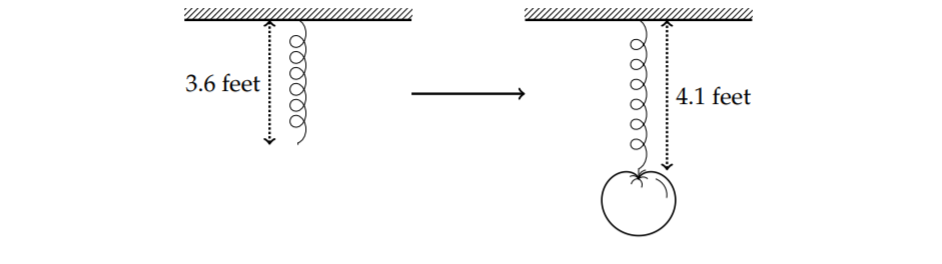
\includegraphics[scale=0.65]{Spring Mass.png}
\end{figure}

\section{}

Let $\mathcal{R}$ be the region in the $x-y$ plane below $y = \text{sec}(x)\text{tan}(x)$ and above $y = -2$ from $x = 0$ to $x = \pi/4$. \\

(a) Write an integral to compute the volume of the solid formed by revolving $\mathcal{R}$ around the line $y = -2$. \\

(b) Evaluate the integral from part (a). 

\section{}

Determine the surface area of the solid obtained by rotating $x = y^3$, $0\leq y \leq 2$ about the $y$-axis. 

\section{}

Determine the center of mass for the plate of constant density $\delta$ on the region bounded by $y = x^3$ and $y = \sqrt{x}$.

\section{}

A tank is formed by revolving the line $y = \frac{15}{4}x$, $0\leq x \leq 4$ about the $y$ - axis (assume the $x$ and $y$ axis are measured in meters). If the tank is filled with water with density 1000 kg/m$^3$, find the work done in pumping all of the water to the top of the tank.

\section*{Answers}

\noindent{1a. $\frac{7}{8}x^{8/7} - 2$arcsin$(x) + C$.}\\
1b. $\frac{\text{sin}(\text{ln}(x))}{3}+C$.\\
1c. $-x^{-1} - \frac{2}{3}x^{-\frac{3}{2}} + C$.\\
1d. $\frac{1}{11}$tan$^{11}(x) + \frac{2}{9}$tan$^9(x) + \frac{1}{7}$tan$^7(x) + C$.\\
1e. $\frac{2}{3}x^3 - x^2 +6x + 13$ln$|x+3| + C$.\\
1f. $-\frac{\pi^{-x}}{\text{ln}(\pi)} + C$.\\
1g. arcsin$(\frac{x-4}{4}) + C$.\\
1h. $\frac{1}{2}x^2e^{2x} - \frac{1}{2}xe^{2x} + \frac{1}{4}e^{2x} +C$.\\

\noindent{2) 1.52 ft-lbs}\\

\noindent{3) $\pi \left(-11/3 + 4\sqrt{2} + \pi\right)$.}\\

\noindent{4) $\frac{\pi}{27}\left(145^{3/2} - 1\right)$.}\\

\noindent{5) $(\overline{x}, \overline{y}) = \left(\frac{12}{25},\frac{3}{7}\right)$.\\

\noindent{6) $W = \int_{y_0}^{y_1} \, \rho g A(y) d \, dy = \int_{0}^{15} (1000)(9.8)[\pi(\frac{4}{15}y)^2](15-y) \, dy \approx 9.23628 \times 10^6 \text{J},$ where $\rho$ is the density of the water, $g$ is gravitational acceleration, $A(y)$ is the area of an arbitrary horizontal cross section, $d$ is the distance an arbitrary cross section is pumped, and $y_0,y_1$ are the lowest and highest cross sectional elevations respectively. 

\end{document}